\chapter{고유 거리, 크루스칼 기하와 지평선 관측자}

슈바르츠실트 계량은 지평선에서 특이해지는 것처럼 보인다. 곡률은 그렇지 않다. 이 두 진술을 구분하기 위해 먼저 블랙홀의 전체 크기를 없앤 다음, 반지름 좌표를 지평선으로부터의 고유 거리로 바꾼다. 지평선 부근에서 이렇게 얻은 기하는 가속 좌표로 표현한 평범한 평탄 시공간이다. 이 기하를 그려 놓으면 앨리스, 밥, 찰리에 관한 질문은 말로만 제기되는 역설이 아니라 세계선과 광선에 관한 문제가 된다.

\section{슈바르츠실트 반지름을 척도에서 제거하기}

나중에 재조정된 변수에 익숙한 기호를 붙일 수 있도록 먼저 프라임이 붙은 좌표로 시작하자:
\begin{equation}
d\tau^2
=
\left(1-\frac{2MG}{r'}\right)dt'^2
-
\frac{dr'^2}{1-\frac{2MG}{r'}}
-
r'^2d\Omega_2^2.
\label{eq:l7-schwarzschild-dimensional}
\end{equation}
슈바르츠실트 반지름과 무차원 좌표를 도입하면
\begin{equation}
r_{\mathrm S}=2MG,
\qquad
r=\frac{r'}{r_{\mathrm S}},
\qquad
t=\frac{t'}{r_{\mathrm S}}.
\label{eq:l7-rescaling}
\end{equation}
여기서는 \(c=1\)를 사용하므로 시간과 길이의 단위가 같다. 따라서 반지름 \(r_{\mathrm S}\)은 길이인 동시에 그 길이를 빛이 가로지르는 데 걸리는 시간이다. 대입하면 다음을 얻는다.
\begin{equation}
d\tau^2
=r_{\mathrm S}^2
\left[
\left(1-\frac1r\right)dt^2
-
\frac{dr^2}{1-\frac1r}
-
r^2d\Omega_2^2
\right].
\label{eq:l7-schwarzschild-rescaled}
\end{equation}
그러므로 회전하지 않고 전하도 없는 모든 슈바르츠실트 블랙홀은 같은 무차원 기하를 갖는다. 질량이 바뀌면 계량에 곱해지는 척도만 달라지고, 대괄호 안 식의 형태는 바뀌지 않는다. 이는 구의 모든 거리를 반지름으로 나눈 뒤 그리는 것과 같다. 같은 그림으로 달과 지구를 나타낼 수 있지만, 각 그림에서 1센티미터가 나타내는 실제 거리는 서로 다르다.

\begin{classroomqa}
\audiencequestion{계량의 반지름 성분과 각도 성분에는 각각 어떤 부호가 붙나요?}
\lecturerresponse{여기서 쓰는 \(+---\) 부호 규약에서는 두 공간 성분 모두 음의 부호를 갖습니다. 식을 적는 동안 강의실에서 그 부호를 짚어 주었지요. 극좌표를 축에서 재는지 적도면에서 재는지에 따라 각도 인자에 사인이나 코사인을 쓸 수 있습니다. 간결한 표기 \(d\Omega_2^2\)를 쓰면 이 규약의 차이를 피할 수 있습니다.
\lecturetimestamp{00:07:48--00:08:12}}
\end{classroomqa}

\section{지평선에서의 곡률 척도}

이 재척도화는 긴 텐서 계산 없이도 중요한 물리적 질문에 답해 준다. 계량 성분은 무차원량이다. 크리스토펠 기호에는 좌표 미분이 한 번 포함되므로 차원은 길이의 역수이고, 물리적 정규직교 틀에서 리만 텐서 성분의 차원은
\begin{equation}
[g_{\mu\nu}]=1,
\qquad
[\Gamma^\mu{}_{\nu\rho}]=L^{-1},
\qquad
[R_{\hat\alpha\hat\beta\hat\gamma\hat\delta}]
=L^{-2}.
\label{eq:l7-curvature-dimensions}
\end{equation}
지평선 \(r=1\)에서는 물리적 길이로 쓸 수 있는 것이 \(r_{\mathrm S}\)뿐이다. 따라서 지평선에서 조석 곡률의 규모는
\begin{equation}
\left|R_{\hat\alpha\hat\beta\hat\gamma\hat\delta}\right|_{\mathrm{hor}}
\sim \frac{1}{r_{\mathrm S}^2}.
\label{eq:l7-horizon-curvature}
\end{equation}
이어야 한다. 더 일반적으로는 \(r_{\mathrm S}^{-2}\)에 \(r\)의 무차원 함수를 곱한 형태로 나타난다. 이 설명은 리만 조석장에 관한 것이며, 슈바르츠실트 진공에서 사라지는 리치 스칼라에 관한 것은 아니다.

물리적 결론은 즉시 얻어진다. 질량이 커지면 \(r_{\mathrm S}\)이 커지고 지평선의 조석장은 약해진다. 작은 블랙홀은 물체가 지평선을 통과할 때 물체를 잡아당겨 찢을 수 있지만, 초대질량 블랙홀의 지평선 부근에서는 조석력이 약할 수 있다. 그럼에도 안쪽으로 갈수록 곡률은 커져 \(r=0\)에서 발산한다. 따라서 지평선과 특이점은 근본적으로 서로 다른 대상이다.

\section{지평선으로부터의 고유 거리}

이후의 국소 계산에서는 \(r_{\mathrm S}=1\)로 둔다. 상대론에서 좌표 변환은 겉모양만 바꾸는 일이 아니다. 부적절한 좌표를 쓰면 특이한 계수가 규칙적인 기하를 가릴 수 있다. 슈바르츠실트 좌표의 차이 \(r-1\)는 지평선으로부터 실제로 측정한 반지름 방향 거리가 아니다.

\begin{figure}[htbp]
\centering
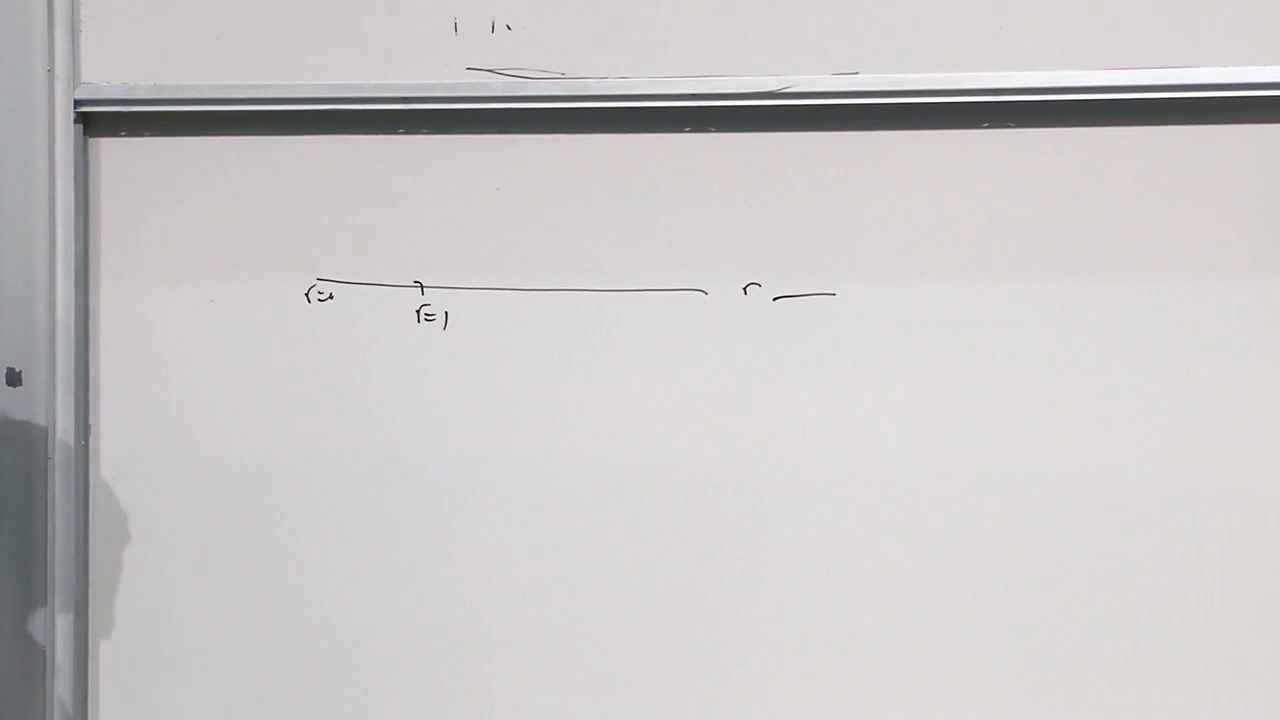
\includegraphics[width=0.78\textwidth]{lecture_07_figure_02.png}
\caption{칠판에 그린 반지름 좌표선. 지평선은 \(r=1\)에 있고, 곡률 특이점은 \(r=0\)에 있다.}
\lectureframe{00:16:11}
\end{figure}

\(t\)와 각도를 고정하자. 그러면 양의 공간 선요소는 다음과 같다.
\begin{equation}
ds^2=\frac{dr^2}{1-\frac1r},
\qquad
ds=\sqrt{\frac{r}{r-1}}\,dr.
\label{eq:l7-radial-proper-line}
\end{equation}
지평선으로부터의 무차원 고유 거리를 다음과 같이 정의하자.
\begin{equation}
\rho(r)
=
\int_1^r\sqrt{\frac{r'}{r'-1}}\,dr'.
\label{eq:l7-rho-definition}
\end{equation}
전체 척도를 복원하면 물리적 거리는 \(r_{\mathrm S}\rho\)이다. 적분의 닫힌 형태는 필요하지 않다. 필요한 것은 그 도함수뿐이다.
\begin{equation}
\frac{d\rho}{dr}
=\sqrt{\frac{r}{r-1}},
\qquad
d\rho^2
=\frac{dr^2}{1-\frac1r}.
\label{eq:l7-rho-derivative}
\end{equation}
따라서 복잡한 반지름 항은 정확히 \(-d\rho^2\)로 바뀐다. 이것이 \(\rho\)를 도입하는 이유다.

이제 시간 좌표를 한 번 더 재척도화한다.
\begin{equation}
\omega=\frac{t}{2}.
\label{eq:l7-omega}
\end{equation}
\(r\)가 \(\rho\)의 함수이므로 계량은 다음과 같이 쓸 수 있다.
\begin{equation}
d\tau^2
=
F(\rho)\rho^2d\omega^2
-
d\rho^2
-
r(\rho)^2d\Omega_2^2.
\label{eq:l7-rho-metric}
\end{equation}

\begin{classroomqa}
\audiencequestion{시간 계수가 \(F(\rho)\rho^2\) 형태가 되도록 \(F(\rho)\)를 그저 정의한 건가요?}
\lecturerresponse{그렇습니다. 이 단계에서 이 인수분해에는 별도의 물리적 의미가 없습니다. 편리한 정의일 뿐입니다. 이 정의가 유용해지는 것은 지평선에서 멀리 떨어진 곳과 가까운 곳에서 \(F\)의 극한을 취할 때입니다.
\lecturetimestamp{00:26:39--00:26:59}}
\end{classroomqa}

멀리 떨어진 곳에서는 슈바르츠실트 시간 계수가 1에 가까워진다. \(dt=2d\omega\)이므로 이는 다음과 같이 된다.
\begin{equation}
\lim_{\rho\to\infty}F(\rho)\rho^2=4.
\label{eq:l7-far-limit}
\end{equation}
지평선 부근에서는 식 ~\eqref{eq:l7-rho-definition}로부터 다음을 얻는다.
\begin{equation}
\begin{aligned}
\rho&\simeq 2\sqrt{r-1},\\
r(\rho)&=1+\frac{\rho^2}{4}+O(\rho^4),\\
\lim_{\rho\to0}F(\rho)&=1.
\end{aligned}
\label{eq:l7-near-expansion}
\end{equation}

\begin{figure}[htbp]
\centering
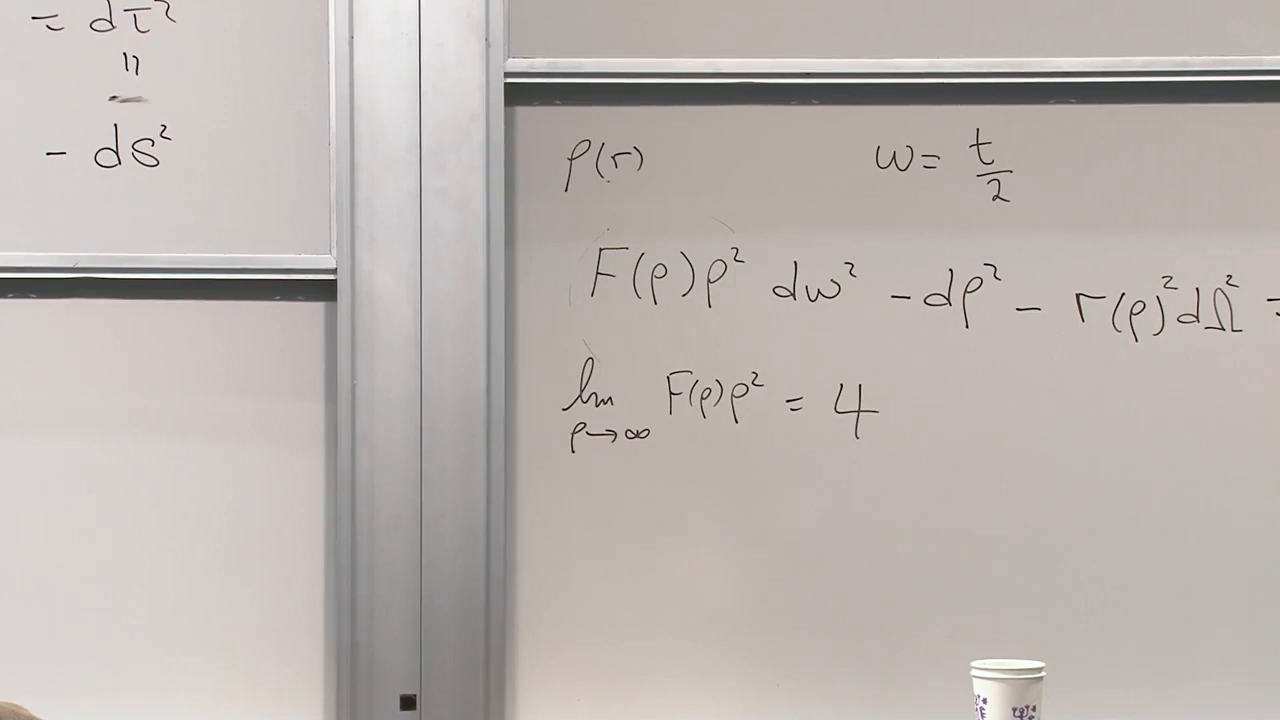
\includegraphics[width=0.90\textwidth]{lecture_07_figure_03.png}
\caption{계량을 \((\rho,\omega)\)로 나타낸 모습, 점근적 시간 계수와 지평선 근처의 극한 \(F\to1\) 및 \(r=1+\rho^2/4+\cdots\).}
\lectureframe{00:37:30}
\end{figure}

\section{지평선에 숨어 있는 평탄 시공간}

\(\rho=0\) 부근에서 식 ~\eqref{eq:l7-rho-metric}의 반지름-시간 부분은 다음과 같이 근사된다.
\begin{equation}
d\tau_{\mathrm{radial}}^2
\simeq
\rho^2d\omega^2-d\rho^2.
\label{eq:l7-rindler-metric}
\end{equation}
이는 쌍곡 극좌표로 나타낸 평탄한 민코프스키 시공간이다. 다음과 같이 정의하자.
\begin{equation}
X=\rho\cosh\omega,
\qquad
T=\rho\sinh\omega.
\label{eq:l7-rindler-transform}
\end{equation}
그러면
\begin{equation}
dT^2-dX^2
=
\rho^2d\omega^2-d\rho^2.
\label{eq:l7-minkowski-check}
\end{equation}
\(\rho\)가 일정한 곡선은 다음 조건을 만족하므로 쌍곡선이다.
\begin{equation}
X^2-T^2=\rho^2
\label{eq:l7-constant-rho}
\end{equation}
\(\omega\)가 일정한 곡선은 원점에서 뻗어 나가는 직선이다. \(\omega\to\infty\)일 때 이 직선들은 영선 \(T=X\)에 가까워진다. 따라서 좌표 시간상 무한대에 놓인 것처럼 보이던 슈바르츠실트 지평선은 규칙적인 도표에서 평범한 영선이다.

\begin{figure}[htbp]
\centering
\includegraphics[width=0.88\textwidth]{lecture_07_figure_06.png}
\caption{완성된 칠판 기하: \(\rho\) 일정 쌍곡선, \(\omega\) 일정 직선, 영지평선, 그리고 그 위쪽의 \(r<1\) 영역.}
\lectureframe{00:38:30}
\end{figure}

\begin{figure}[htbp]
\centering
\resizebox{0.96\linewidth}{!}{%
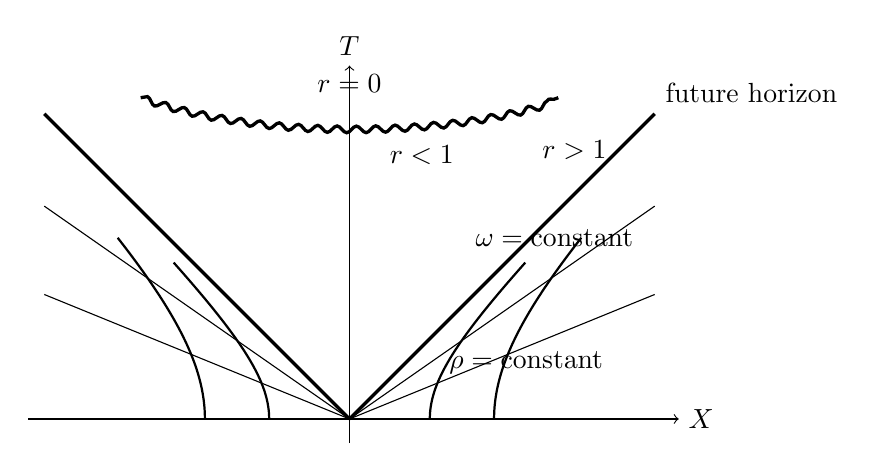
\begin{tikzpicture}[scale=1.02]
\draw[->] (-4.0,0) -- (4.1,0) node[right] {$X$};
\draw[->] (0,-0.3) -- (0,4.4) node[above] {$T$};
\draw[very thick] (0,0) -- (3.8,3.8)
  node[above right] {future horizon};
\draw[very thick] (0,0) -- (-3.8,3.8);
\draw[thick]
  plot[domain=0:1.42,samples=50]
  ({1.0*cosh(\x)},{1.0*sinh(\x)});
\draw[thick]
  plot[domain=0:1.05,samples=50]
  ({1.8*cosh(\x)},{1.8*sinh(\x)});
\draw[thick]
  plot[domain=0:1.42,samples=50]
  ({-1.0*cosh(\x)},{1.0*sinh(\x)});
\draw[thick]
  plot[domain=0:1.05,samples=50]
  ({-1.8*cosh(\x)},{1.8*sinh(\x)});
\draw[thin] (0,0) -- (3.8,1.55);
\draw[thin] (0,0) -- (3.8,2.65);
\draw[thin] (0,0) -- (-3.8,1.55);
\draw[thin] (0,0) -- (-3.8,2.65);
\draw[very thick,decorate,decoration={snake,amplitude=1.2pt,segment length=7pt}]
  (-2.6,4.0) .. controls (-1.2,3.5) and (1.2,3.5) .. (2.6,4.0);
\node at (0,4.18) {$r=0$};
\node at (2.2,0.7) {$\rho=\mathrm{constant}$};
\node at (2.55,2.25) {$\omega=\mathrm{constant}$};
\node at (0.9,3.28) {$r<1$};
\node at (2.8,3.35) {$r>1$};
\end{tikzpicture}
}
\caption{인과 구조를 깨끗하게 복원한 그림. 지평선은 영선이고, 곡률 특이점 \(r=0\)은 블랙홀 내부의 미래 경계다.}
\label{fig:l7-kruskal-clean}
\end{figure}

\(\rho\)가 작아지는 극한은 유클리드 극좌표에서 반지름이 작아지는 극한과 다르다. 작은 유클리드 원은 한 점으로 수축한다. 반면 \(\rho\)가 일정한 쌍곡선은 하나의 영선 전체에 가까워진다. 따라서 \(\rho=0\)은 축이 만나는 점만이 아니라 지평선 전체를 나타낸다.

외부 영역의 식을 \(r<1\)까지 해석적 연장할 수 있다. 지평선 부근에서는 \(r-1\simeq\rho^2/4\)이므로 내부 영역은 형식적으로 \(\rho^2<0\)에 해당한다. \(\rho\)을 허수라고 부를 수도 있지만, \(\rho^2\), \(r\) 또는 규칙적인 좌표 \(T,X\)를 쓰는 편이 더 깔끔하다. 내부에서는 슈바르츠실트 계수 \(t\)와 \(r\)의 부호가 서로 바뀐다. 그렇다고 물리적 손목시계가 자로 변한다는 뜻은 아니다. 슈바르츠실트 좌표의 인과적 성격이 서로 바뀌었다는 뜻이다.

\begin{classroomqa}
\audiencequestion{지평선 안쪽에 있는 수평 쌍곡선은 무엇이고, 직선 광선은 무엇인가요?}
\lecturerresponse{쌍곡선은 일정한 \(r\), 즉 일정한 \(\rho^2\)인 곡선을 \(r<1\)까지 연장한 것입니다. 직선은 슈바르츠실트 시간이 일정한 곡선입니다. 외부에서는 유용한 좌표 격자를 이루지만, 내부에서는 같은 표지를 물리적 관측자의 궤적으로 오해해서는 안 됩니다.
\lecturetimestamp{00:44:12--00:44:59}}
\end{classroomqa}

\begin{classroomqa}
\audiencequestion{수직 방향은 시간 좌표인가요? 그렇다면 어떤 기준틀을 나타내나요?}
\lecturerresponse{새 시공간도에서 수직 방향은 정칙적인 시간 방향이지만, 특이한 슈바르츠실트 시간 \(t\)은 아니다. 이 도표는 자유낙하하는 인과 구조에 맞춰져 있다. 외부에서 반지름을 고정한 채 정지해 있는 관측자는 쌍곡선을 따라가며 가속해야 한다. 자유낙하하는 관측자는 영지평선을 매끄럽게 통과한다.
\lecturetimestamp{00:45:54--00:46:48}}
\end{classroomqa}

\begin{classroomqa}
\audiencequestion{내부에서 \(\rho^2<0\)이라면, \(i\)라는 명시적인 인수는 어디에 있나요?}
\lecturerresponse{허수 \(\rho\)를 도입할 수 있지만, 그렇게 해도 얻는 것은 없다. 불변인 물리적 내용은 \(r\), \(\rho^2\), 그리고 실수인 규칙적 좌표 \(T,X\)에 담겨 있다. 관계식 \(r-1\simeq\rho^2/4\)은 지평선 근처에서만 성립하는 전개다.
\lecturetimestamp{00:52:35--00:53:00}}
\end{classroomqa}

강의에서는 흔히 이 규칙적인 도표를 크루스칼 그림이라고 부른다. 엄밀히 말하면 정확한 크루스칼 좌표에는 전체 슈바르츠실트 계량을 규칙적으로 유지하는 반지름 인자가 포함되지만, 식 ~\eqref{eq:l7-rindler-transform}는 그 계량의 지평선 근처 형태다. 인과 구조에 관한 핵심은 같다. 지평선은 매끄럽지만, 내부의 미래 방향 시간꼴 곡선이나 영곡선은 모두 \(r=0\)에서 끝난다. 어떤 초광속 회전도 그 곡선을 지평선을 거슬러 되돌아가게 할 수 없다.

\subsection{좌표 특이성은 어떻게 이해되었나}

원래의 슈바르츠실트 좌표에서는 계량 계수가 특이해 보이므로 지평선이 매끄럽다는 사실을 역사적으로 알아보기가 어려웠다. 에딩턴과 이후의 핀켈슈타인은 지평선을 가로질러 쓸 수 있는 좌표를 도입했고, 핀켈슈타인은 한 방향으로만 통과할 수 있는 인과적 경계를 알아보았다. 플라스마 물리학 연구를 통해 좌표 변환에 능숙했던 크루스칼은 영원한 해의 전역적이고 규칙적인 그림을 제시했다.

강의는 이어서 ‘블랙홀’이라는 표현이 널리 쓰이도록 하는 데 기여한 존 휠러에 관한 이야기를 잠시 나눈다. 이 회고에는 역사적 의미뿐 아니라 개인적인 면도 담겨 있다. 핵 경쟁을 포함한 정치적 판단에서 견해가 크게 달랐던 경우에도 휠러는 다정하고 사려 깊은 친구로 기억된다. 휠러를 사교적 관습에 얽매인 사람으로만 보는 고정관념을 깨기 위해 유쾌한 개인 일화도 소개한다. 기술적인 논점은 ‘블랙홀에는 털이 없다’는 응수로 되돌아온다. 교란된 비회전 블랙홀은 빠르게 구대칭 상태에 가까워지고, 회전하는 블랙홀은 보존되는 매개변수들이 정하는 정상 상태의 형태로 가라앉는다. 이는 무모 정리 전체에 대한 증명이 아니라 강의에서 제시하는 무모 아이디어의 정성적 설명이다.

\section{앨리스는 통과하고 밥은 바깥에 머문다}

최대 연장 도표에는 통상적인 초기 조건에서 별이 붕괴해 생기는 단순한 시공간에는 나타나지 않는 영역들이 들어 있다. 관측자 사고 실험에서는 외부 영역, 미래 지평선, 블랙홀 내부만 사용한다.

\begin{figure}[htbp]
\centering
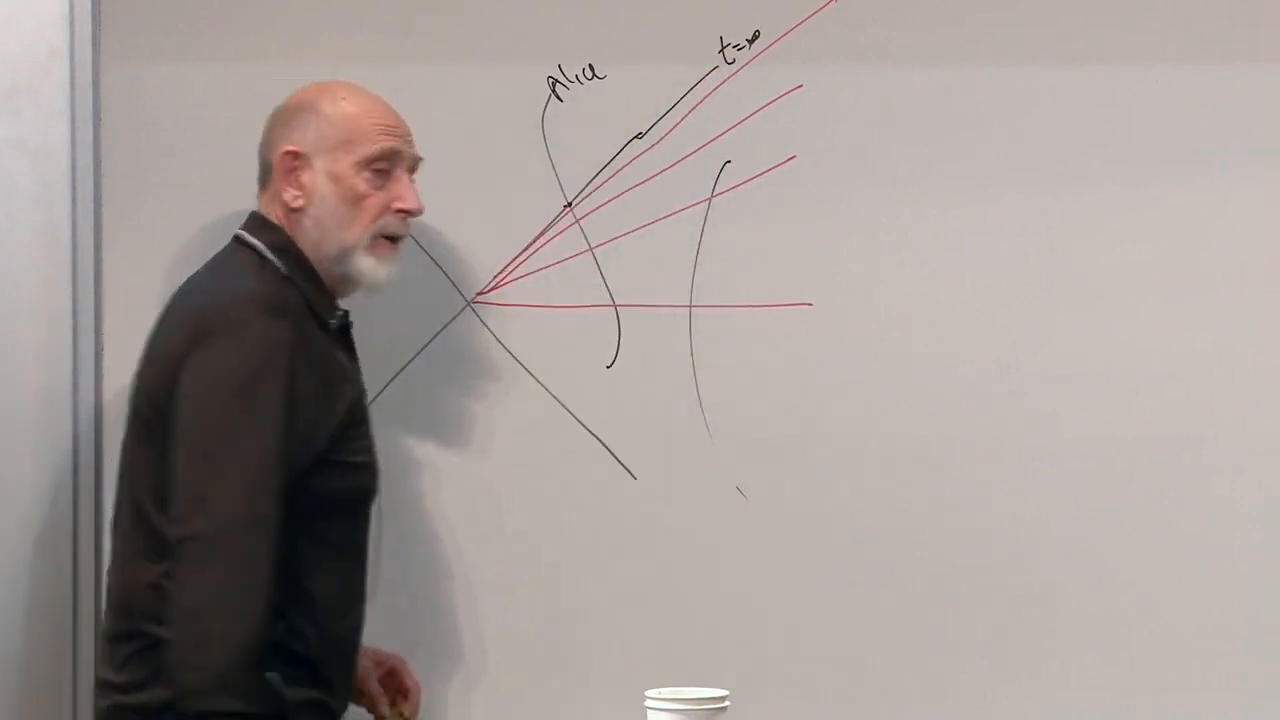
\includegraphics[width=0.84\textwidth]{lecture_07_figure_04.png}
\caption{앨리스의 낙하 세계선과 슈바르츠실트 시간이 일정한 광선들. 극한 광선에는 \(t=\infty\)이라는 표지가 붙어 있다.}
\lectureframe{00:54:54}
\end{figure}

앨리스는 자유낙하한다. 그녀의 세계선은 지평선을 통과해 유한한 고유 시간 안에 특이점에 도달한다. 블랙홀이 충분히 커서 지평선의 조석력이 작다면, 지평선을 통과할 때 그녀의 시계에는 아무런 특이한 일도 일어나지 않는다.

반면 밥은 외부에서 반지름을 고정한 채 머문다. 그 위치를 유지하려면 가속해야 한다. 앨리스의 궤적에서 더 늦은 시점에 나온 빛은 점점 더 큰 지연과 적색편이를 거쳐 그에게 도달한다. 슈바르츠실트 시간으로 보면 앨리스는 \(t=\infty\)에 가까워지고, 밥은 그녀가 지평선을 통과한 뒤에 방출한 신호를 전혀 받지 못한다. 이는 인과적 신호와 외부의 시간 절단에 관한 진술이지, 지평선에 물질 표면이 있다는 증거가 아니다.

\begin{classroomqa}
\audiencequestion{밥이 앨리스가 느려지는 것을 본다면 앨리스는 밥이 빨라지는 것을 봐야 하나요?}
\lecturerresponse{아닙니다. 앨리스는 자신의 세계선이 지속되는 동안 밥의 평범한 광신호를 계속 받는다. 밥의 세계선에는 그녀에게 도달할 수 있는 마지막 사건이 있지만, 그 사건이 마지막인 것은 그 뒤에 앨리스가 특이점에 도달하기 때문이다. 밥에게 갑작스러운 일은 일어나지 않는다. 관측은 언제나 과거 광원뿔을 들여다보며, 두 세계선 사이에는 비대칭적인 인과 관계가 있다.
\lecturetimestamp{00:58:31--01:01:23}}
\end{classroomqa}

\begin{classroomqa}
\audiencequestion{밥의 좌표로 앨리스가 아직 지평선 가까이에 있음을 안다면, 밥은 내려가 그녀를 구한 뒤 돌아올 수 있나요?}
\lecturerresponse{구조를 위한 세계선은 앨리스가 사건 지평선을 통과하기 전에 그녀와 만나야 한다. 그 사건 이후에는 미래 방향 경로 가운데 그녀를 만나 외부로 되돌아올 수 있는 경로가 없다. 슈바르츠실트 시간 절단에서는 통과가 \(t=\infty\)에 놓인다고 해서 앨리스가 구조할 수 있는 물질 표면 위에 계속 앉아 있는 것은 아니다. 이는 그 절단으로는 지평선 너머까지 아우르는 전역적인 ‘현재’를 정의할 수 없음을 보여 준다.
\lecturetimestamp{01:01:24--01:02:12}}
\end{classroomqa}

\section{찰리는 앨리스를 따라간다}

찰리가 앨리스보다 조금 뒤에서 낙하한다고 하자. 그러면 두 사람은 지평선 부근에서 거의 관성 운동을 한다. 서로 신호를 주고받고, 양방향으로 대화하거나 손을 잡을 수도 있다. 어느 쪽도 지평선을 표시하는 표지판을 발견하지 못한다. 밥과 다른 점은 세 사람의 이름에 있는 것이 아니다. 자유낙하와 외부에 머물기 위해 가속하는 세계선의 차이다.

\begin{classroomqa}
\audiencequestion{농구공이 골대를 따라가듯 앨리스가 먼저 낙하하고 찰리가 뒤따르면, 밥에게는 어떻게 보이나요?}
\lecturerresponse{밥은 두 사람이 모두 지평선에 가까워지는 것을 본다. 앞서 있는 앨리스가 먼저 점점 느려지고 반지름 방향으로 압축되는 것처럼 보인다. 찰리는 그녀 바로 뒤에 점점 가까워지는 듯 보이지만, 밥이 외부에서 극한적으로 관측할 때는 결코 따라잡지 못한다. 이렇게 시각적으로 쌓여 보인다고 해서 어느 낙하자가 실제로 그렇게 느낀다는 뜻은 아니다.
\lecturetimestamp{01:04:12--01:06:05}}
\end{classroomqa}

\begin{classroomqa}
\audiencequestion{낙하자는 조석력에 의해 반지름 방향으로 늘어나야 하는데, 납작해져 보인다는 설명과 모순되지 않나요?}
\lecturerresponse{서로 다른 효과다. 납작해 보이는 것은 밥의 슈바르츠실트 좌표를 사용한 묘사에 해당한다. 조석 신장 효과는 앨리스와 찰리가 느낄 수 있는 국소 곡률 효과다. 관측자들에 관한 설명은 블랙홀이 충분히 크거나 관측자들이 충분히 작아서 지평선의 조석 효과가 무시할 수 있을 정도라고 가정한다. 태양 질량 정도의 블랙홀에서는 지평선 조석력이 매우 강하지만, 초대질량 블랙홀에서는 약할 수 있다.
\lecturetimestamp{01:06:07--01:08:18}}
\end{classroomqa}

\begin{classroomqa}
\audiencequestion{찰리는 아직 외부에 있는 동안 앨리스가 통과하는 것을 보나요?}
\lecturerresponse{영선을 그려 보자. 앨리스가 통과하는 순간 방출된 빛은 지평선을 따라가 찰리가 통과할 때 그에게 도달한다. 그 사건에서 찰리는 자신이 앨리스의 통과를 보았다고 계산할 수 있지만, 어느 관측자도 국소적인 표지를 마주치지는 않는다. 그 뒤에는 찰리가 내부에 있는 앨리스를 볼 수 있다. 통과하기 전에 가속해 멀어지고 외부에 계속 머무는 데 성공한다면, 찰리는 그 통과 장면을 결코 보지 못한다.
\lecturetimestamp{01:08:19--01:11:11}}
\end{classroomqa}

\begin{classroomqa}
\audiencequestion{앨리스가 이미 내부에 있고 찰리는 외부에 있다면, 나중에 두 사람의 반지름과 통과 시각을 어떻게 비교할 수 있나요?}
\lecturerresponse{‘동시에’라는 말만으로는 관측자와 무관한 동시성 관계를 알아낼 수 없다. 앨리스는 자신의 과거 광원뿔에 찰리를 두고 있으며, 자신이 더 안쪽으로 들어가야 찰리가 나중에 통과하는 것을 볼 수 있다. 구체적인 세계선과 영선이 이 질문에 답해 준다. 서로 멀리 떨어진 여러 낙하자에게 이 결론을 일반화하려면 보편적인 통과 시각이 있다고 가정하지 말고, 실제 인과 도표를 그려 확인해야 한다.
\lecturetimestamp{01:11:14--01:12:31}}
\end{classroomqa}

규칙적인 지평선 근처 좌표에서 자유낙하 궤적은 거의 직선이다. 전체 슈바르츠실트 기하에서 정확히 직선인 것은 아니지만, 약한 곡률을 가진 큰 블랙홀의 지평선 부근에서는 근사가 잘 맞는다.

\begin{classroomqa}
\audiencequestion{블랙홀 내부의 양자 중력 영역에서 일어나는 일을 끈 이론으로 밝힐 수 있나요?}
\lecturerresponse{바로 그 지점에서 주제가 미묘해진다. 특이점 부근에는 양자 중력 이론이 필요하고 끈 이론은 하나의 후보 틀이지만, 관련 문제들은 고전적인 도표를 단순히 적용해서 해결되는 것이 아니라 당시에도 활발히 연구 중인 어려운 문제였다.
\lecturetimestamp{01:13:04--01:13:38}}
\end{classroomqa}

\begin{classroomqa}
\audiencequestion{앨리스가 통과할 때 그녀의 시계와 속도에는 어떤 일이 일어나나요?}
\lecturerresponse{그녀의 시계는 국소적인 보통 속도로 계속 가며 유한한 고유 시간을 기록한다. 순간 정지계에서는 그녀가 정지해 있고, 국소 자유낙하계에 대해서는 평범하고 유한한 속도를 갖는다. 큰 블랙홀의 지평선 부근 기하는 거의 평탄하므로, 특이점 부근에서 곡률이 강해질 때까지 그녀의 세계선에 표시한 같은 고유 시간 간격들은 계속 규칙적이다.
\lecturetimestamp{01:13:39--01:14:44}}
\end{classroomqa}

\begin{classroomqa}
\audiencequestion{밥이 바깥쪽으로 가속하지만 낙하를 피할 만큼 충분히 가속하지 못하면 어떻게 되나요?}
\lecturerresponse{그러면 그의 세계선은 바깥쪽으로 휘지만 결국 지평선을 통과한다. 매우 늦게 통과한다면 앨리스가 통과한 직후의 모습을 볼 수 있지만, 특이점에 도달하기까지 남은 고유 시간은 짧다. 스케치에서 세계선의 기울기는 보정된 자나 시계가 아니다. 그려진 유클리드 길이가 아니라 인과적 순서가 의미를 유지한다.
\lecturetimestamp{01:14:47--01:16:31}}
\end{classroomqa}

이 모든 결론은 어떤 신호도 빛보다 앞서지 않는다고 가정한다. 강의에서는 이탈리아에서 중성미자가 겉보기에 초광속으로 측정되었다는 당시의 언론 보도를 잠깐 농담 삼아 언급한다. 이는 상대론의 예외가 아니라 실험 시간 측정의 오류를 가리킨다. 인과 구조는 그 자체로 영선에 의해 제한된다.

\begin{classroomqa}
\audiencequestion{앨리스가 지평선 쪽으로 잠수했다가 돌아오면, 앨리스와 밥이 가지고 간 동기화된 시계로 이 문제를 판별할 수 있나요?}
\lecturerresponse{두 사람은 만났을 때 시계를 비교할 수 있지만, 세계선이 갈라진 뒤에는 특히 한 사람이 운동 상태를 바꾸면 멀리 떨어진 두 시계를 동기화하는 유일한 방법이 없다. 두 세계선을 그리고 주고받은 영선도 표시해야 한다. 그 도표가 구체적으로 정한 실험에 대한 조작적 답을 제공한다.
\lecturetimestamp{01:17:34--01:18:25}}
\end{classroomqa}

\begin{figure}[htbp]
\centering
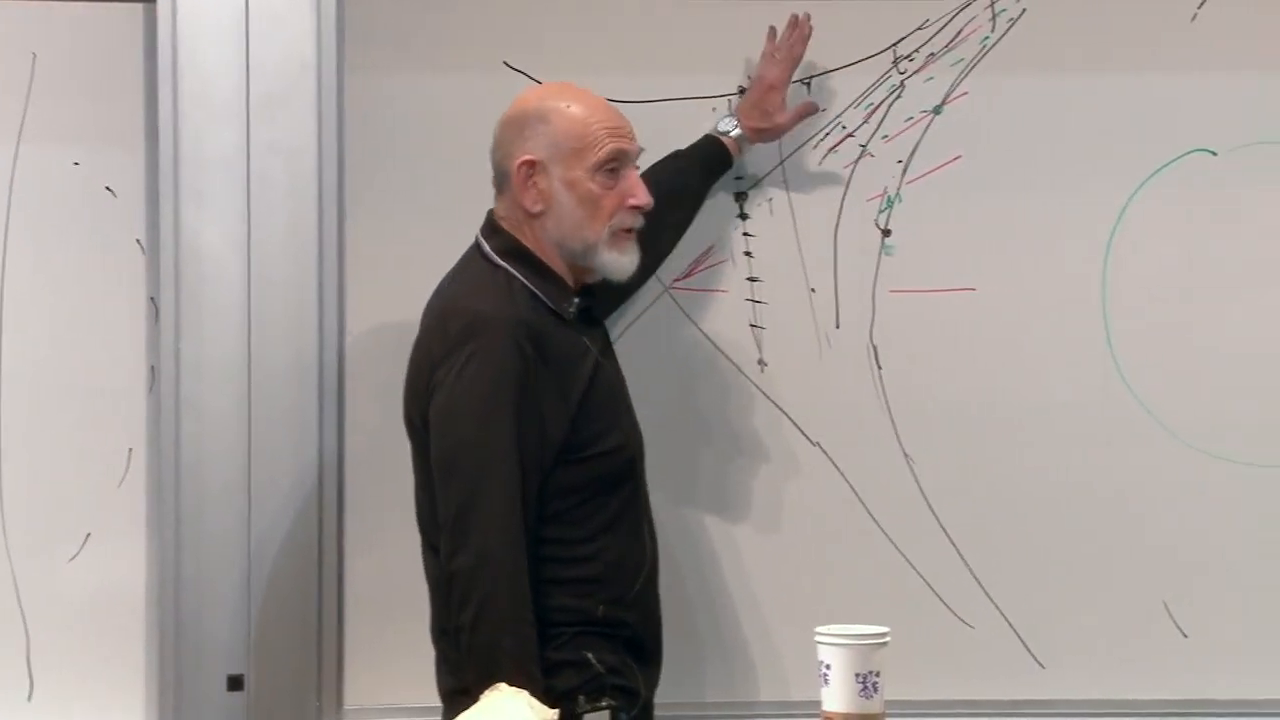
\includegraphics[width=0.86\textwidth]{lecture_07_figure_05.png}
\caption{앨리스, 밥, 찰리에 관한 질문에 답할 때 사용한 전체 인과 도표. 관측되는 사건에서 관측자의 세계선까지 영선을 따라가면 각 관측의 위치를 찾을 수 있다.}
\lectureframe{01:18:12}
\end{figure}

\begin{figure}[htbp]
\centering
\resizebox{0.96\linewidth}{!}{%
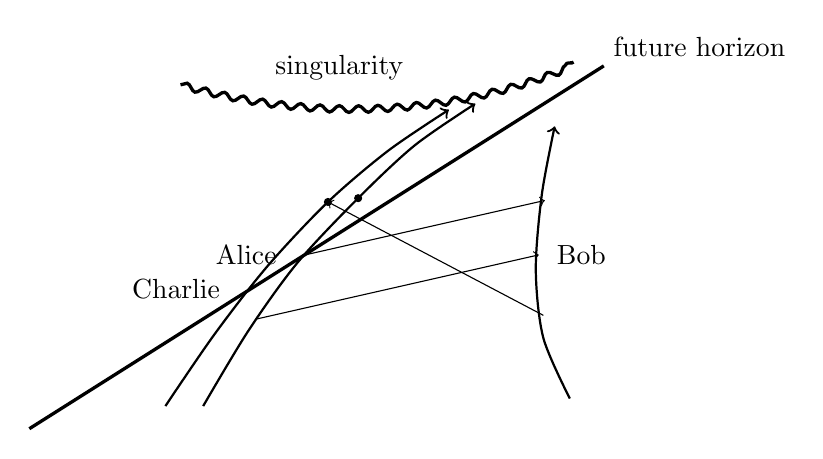
\begin{tikzpicture}[scale=0.96]
\draw[very thick] (-3.8,-0.3) -- (3.8,4.5);
\node[above right] at (3.8,4.5) {future horizon};
\draw[very thick,decorate,decoration={snake,amplitude=1.2pt,segment length=7pt}]
  (-1.8,4.25) .. controls (0.1,3.72) and (2.0,3.92) .. (3.4,4.55);
\node at (0.3,4.48) {singularity};
\draw[thick,->]
  plot[smooth] coordinates {(-1.5,0.0) (-0.9,1.0) (-0.25,1.9)
  (0.55,2.75) (1.3,3.45) (2.1,4.0)};
\node[left] at (-0.4,2.0) {Alice};
\draw[thick,->]
  plot[smooth] coordinates {(-2.0,0.0) (-1.35,0.95) (-0.65,1.85)
  (0.15,2.7) (0.95,3.38) (1.75,3.92)};
\node[left] at (-1.15,1.55) {Charlie};
\draw[thick,->]
  plot[smooth] coordinates {(3.35,0.1) (3.0,0.9) (2.9,1.8)
  (2.98,2.8) (3.15,3.7)};
\node[right] at (3.05,2.0) {Bob};
\draw[thin,->] (-0.8,1.15) -- (2.94,2.0);
\draw[thin,->] (-0.15,2.0) -- (3.02,2.72);
\draw[thin,->] (3.0,1.2) -- (0.15,2.7);
\draw[fill] (0.55,2.75) circle (1.3pt);
\draw[fill] (0.15,2.7) circle (1.3pt);
\end{tikzpicture}
}
\caption{관측자를 나타낸 개략도. 밥이 외부에서 관측하는 경우와 앨리스와 찰리가 서로 관측하는 경우는 서로 다른 영선 구성이지, 서로 주고받는 시계에 관한 구호가 아니다.}
\label{fig:l7-observers-clean}
\end{figure}

\begin{classroomqa}
\audiencequestion{밥은 무한한 시간 동안 앨리스를 보나요? 그렇다면 밥의 현실에서는 그녀가 죽지 않는다는 뜻인가요?}
\lecturerresponse{밥은 자신의 시간으로 끝없이 이어지는 구간 동안 앨리스의 신호를 받지만, 그녀의 시계가 0에 가까운 속도로 느려지는 것을 보며 그녀가 통과하기 전에 방출한 심장 박동 신호는 유한한 개수만 받는다. ‘현실’이라는 말은 국소 사건과 관측자의 점근적 기록 사이의 차이를 가린다. 앨리스는 지평선에서 시계가 멈추는 일을 겪지 않으며, 밥의 기록에는 점점 더 큰 지연과 적색편이가 나타난다.
\lecturetimestamp{01:18:32--01:20:59}}
\end{classroomqa}

\begin{classroomqa}
\audiencequestion{앨리스는 통과한 뒤, 지평선에서 얼어붙은 것처럼 보이던 과거의 모든 물질을 갑자기 보게 되나요?}
\lecturerresponse{갑자기 시야가 트이는 일은 없다. 낙하하는 동안 과거의 물질을 보게 해 주는 과거 광원뿔은 연속적으로 변한다. 그녀는 지금 도달한 빛이 더 일찍 방출되었고 그 물질이 자신보다 먼저 통과했다는 것을 추론할 수 있다. 찰리에게 보이는 앨리스의 모습도 같은 점을 보여 준다. 어느 쪽의 통과도 국소적인 불연속을 일으키지 않으며, 숨겨진 의자나 공룡 더미를 드러내지도 않는다.
\lecturetimestamp{01:21:02--01:23:48}}
\end{classroomqa}

\begin{classroomqa}
\audiencequestion{낙하자가 실제로 보게 될 모습을 현실적으로 시뮬레이션한 영상이 있나요?}
\lecturerresponse{강의에서는 앤드루 해밀턴의 블랙홀 시각화 자료를 소개한다. 이 자료는 들어오는 빛의 큰 광행차와 주파수 이동을 보여 줄 수 있지만, 이해를 돕기보다 더 혼란스럽게 만들 수도 있다. ‘지평선에서 특별한 일은 없다’는 말은 국소 기하에 관한 것이지, 하늘이 평범하게 보인다는 뜻은 아니다.
\lecturetimestamp{01:24:11--01:25:29}}
\end{classroomqa}

\section{영원한 블랙홀에서 성장하는 블랙홀로}

최대 연장된 영원한 블랙홀 도표의 아래쪽 꼭짓점은 별의 붕괴로 형성된 블랙홀에는 직접적인 의미가 거의 없다. 붕괴로 생기는 단순한 기하에는 외부 영역, 미래 지평선, 미래 내부를 포함한 부분만 나타난다. 물질이 블랙홀의 질량을 바꿀 수 있게 되면 이 구분이 중요해진다.

\begin{classroomqa}
\audiencequestion{이상화된 도표의 아래쪽 꼭짓점은 어떤 물리적 사건을 나타내나요?}
\lecturerresponse{영원한 블랙홀의 수학적 해에서는 그 꼭짓점이 최대 연장의 일부다. 물질이 붕괴해 형성된 블랙홀에는 그 아래쪽 영역 전체가 들어 있지 않다. 그 블랙홀의 지평선에는 형성 과정이 있으며, 이를 설명하려면 다른 전역 도표가 필요하다. 이 내용은 다음 강의에서 다룬다.
\lecturetimestamp{01:25:59--01:26:52}}
\end{classroomqa}

작은 시험 물체가 낙하할 때는 그 물체의 역반응을 무시할 수 있으므로 고정된 슈바르츠실트 도표로 충분하다. 상당한 질량의 물체가 낙하하면 블랙홀의 질량과 슈바르츠실트 반지름이 증가한다.
\begin{equation}
r_{\mathrm S}=2GM,
\qquad
\Delta r_{\mathrm S}=2G\,\Delta M.
\label{eq:l7-growing-radius}
\end{equation}
지평선은 다가오는 물체 쪽으로 변형되고, 두 지평선이 합쳐진 뒤 변형된 공통 지평선은 빠르게 안정된 상태로 가라앉는다. 회전하지 않는다고 이상화한 강의에서는 마지막에 조금 더 큰 구가 남는다. 실제 병합에서는 중력파로 에너지도 방출되며, 일반적으로 회전하는 블랙홀이 남는다.

\begin{classroomqa}
\audiencequestion{물질이 낙하해 지평선이 커지면, 예전 지평선 부근에서 얼어붙은 것처럼 보이던 물질을 만나도록 지평선이 바깥으로 움직이나요?}
\lecturerresponse{낙하하는 물체의 질량이 충분히 크면 시험 입자 근사는 더는 유효하지 않다. 지평선은 변형되어 낙하 물체의 포획 영역과 합쳐진 다음 더 큰 정상 지평선으로 이완된다. 사건 지평선의 정확한 위치는 전역적인 성질이므로 낙하 물질이 도착하기 전의 영역까지 뻗을 수 있다. 강의에서는 이 구성을 의도적으로 미루고 다음 시간에 다루기로 한다.
\lecturetimestamp{01:26:55--01:29:05}}
\end{classroomqa}

\begin{classroomqa}
\audiencequestion{물질이 지평선에 도달하는 데 슈바르츠실트 시간으로 무한히 걸린다면서 천문학자들은 어떻게 섬광을 관측하나요?}
\lecturerresponse{밝은 복사는 지평선 자체에서 나오지 않는다. 강착 흐름이나 원반의 기체가 지평선 바깥에서, 광자 궤도가 강하게 휘는 부근을 포함해, 충돌하고 가열된다. 이 외부 플라스마가 우리에게 도달하는 빛을 방출할 수 있다. 빈 슈바르츠실트 기하는 인과 문제를 분리해 보여 주지만 천체물리학적 환경을 온전히 모형화하지는 않는다.
\lecturetimestamp{01:29:07--01:30:22}}
\end{classroomqa}

특성 완화 시간은 빛이 블랙홀을 가로지르는 데 걸리는 시간으로 정해진다.
\begin{equation}
t_{\mathrm{cross}}\sim\frac{r_{\mathrm S}}{c},
\qquad
t_{\mathrm{relax}}\sim
\text{a few to a few tens of }t_{\mathrm{cross}}.
\label{eq:l7-relaxation-scale}
\end{equation}
강의에서는 \(10^{-5}\,\mathrm{s}\)를 킬로미터 규모 블랙홀을 빛이 가로지르는 시간으로 추산하고, 작은 블랙홀의 병합이 거의 정상 상태에 이르기까지는 대략 \(10^{-3}\,\mathrm{s}\)이 걸린다고 추산한다. 태양 질량의 십억 배인 블랙홀에서는 이에 해당하는 시간이 수분에서 수시간에 이른다. 이는 규모를 가늠하기 위한 추산이지 정밀한 병합 계산은 아니다. 여기서 중요한 것은 기하학적 변화의 순서다. 아령 모양에서 땅콩 모양으로, 이어 거의 구형을 거쳐 정상 상태에 이른다.

\begin{classroomqa}
\audiencequestion{변형되었거나 막 병합된 지평선은 얼마나 빨리 안정되나요?}
\lecturerresponse{블랙홀을 빛이 가로지르는 데 걸리는 시간보다 훨씬 길지 않은 시간 척도에서 안정됩니다. 모든 길이와 시간이 \(r_{\mathrm S}\)에 비례하므로, 작은 블랙홀은 초의 몇 분의 일 만에 안정되고 초대질량 블랙홀은 훨씬 긴 시간에 걸쳐 안정됩니다. 무모 정리는 정상 상태의 최종 상태를 설명하며, 과도적인 변형은 중력파를 통해 에너지를 내보냅니다.
\lecturetimestamp{01:30:26--01:33:18}}
\end{classroomqa}

\begin{classroomqa}
\audiencequestion{예전 지평선과 새 지평선 사이에 앞서 떨어진 물질이 있고, 그와 동시에 또 다른 무거운 물체가 낙하한다면 밥에게는 어떻게 보이나요?}
\lecturerresponse{두 정적 슈바르츠실트 도표를 이어 붙여서는 이 질문에 일관되게 답할 수 없다. 시간에 따라 변하는 붕괴 기하를 풀거나 구성하고 그 전역 지평선을 찾아야 한다. 강의에서는 이 질문을 남겨 둔 채 다음 주로 답을 미룬다. 다음 주제는 지평선의 형성이다.
\lecturetimestamp{01:33:20--01:35:41}}
\end{classroomqa}

\section{척도가 바뀌면 무엇이 달라지는가?}

\(r_{\mathrm S}\)이 달라져도 무차원 도표는 변하지 않는다. 그러나 그려진 간격이 물리적으로 뜻하는 바는 달라진다.
\begin{equation}
d\tau_{\mathrm{physical}}^2
=
r_{\mathrm S}^2\,d\hat{\tau}^2,
\qquad
\ell_{\mathrm{physical}}
=
r_{\mathrm S}\,\hat{\ell}.
\label{eq:l7-scale-restoration}
\end{equation}
킬로미터 규모 블랙홀에서 반 킬로미터를 나타내는 무차원 간격은 그보다 십억 배 큰 블랙홀에서는 대략 오억 킬로미터를 나타낸다. 같은 크기로 그린 구들의 비유를 다시 떠올려 보자. 모양은 그대로지만, 선 하나가 나타내는 미터 막대의 수는 반지름에 비례해 커진다.

\begin{classroomqa}
\audiencequestion{슈바르츠실트 반지름이 바뀌면 인과 도표는 어떻게 달라지나요?}
\lecturerresponse{반지름을 척도에서 제거하면 도표는 바뀌지 않는다. 도표에 대응하는 모든 물리적 길이와 시간에는 \(r_{\mathrm S}\)를 곱하고, 대응하는 무차원 위치에서의 곡률에는 \(r_{\mathrm S}^{-2}\)를 곱한다.
\lecturetimestamp{01:35:41--01:38:10}}
\end{classroomqa}

\begin{classroomqa}
\audiencequestion{Bob이 한 각도 위치에 정지해 있지 않고 궤도 운동을 해도 인과적 결론은 같나요?}
\lecturerresponse{적색편이와 신호의 도착 방향은 더 복잡해지지만, 지평선이 만드는 인과적 분리는 달라지지 않는다. 지평선 안에서 방출된 신호를 받는 외부의 시간꼴 궤도는 없다.
\lecturetimestamp{01:38:12--01:38:26}}
\end{classroomqa}

\begin{classroomqa}
\audiencequestion{구형 껍질 내부에서는 중력이 사라지는데, 블랙홀의 질량이 지평면에 퍼져 있으므로 지평선 안에서도 중력이 사라지나요?}
\lecturerresponse{아니다. 사건지평선은 질량을 지닌 물질 껍질이 아니다. 따라서 뉴턴의 껍질 정리는 사건지평선에 적용되지 않는다. 강의에서는 정적 외부 해를 곡률 특이점에 놓인 점원과 비교한다. 그러나 형성 과정에서 현재 낙하 중인 물질을 다루려면 시간에 따라 변하는 기하가 필요하며, 이는 다음 강의에서 다룬다.
\lecturetimestamp{01:38:28--01:40:41}}
\end{classroomqa}

\section{회전과 방사 방향 기하}

각운동량은 붕괴 후에도 남는다. 회전하는 블랙홀의 외부 기하는 슈바르츠실트 시공간과 다르다. 그 정상해는 커 해이고, 회전은 지평선의 기하를 변형시키며, 틀 끌림은 관성 방향을 블랙홀 주위로 끌고 간다. 원칙적으로는 이러한 외부 중력 효과를 측정해 각운동량을 알아낼 수 있다. 각운동량을 가진 물질은 지평선을 통과한다고 해서 각운동량을 잃지 않는다.

\begin{classroomqa}
\audiencequestion{블랙홀의 각운동량을 측정할 수 있나요? 회전은 외부 중력을 바꾸나요?}
\lecturerresponse{그렇다. 각운동량은 보존되는 매개변수로 남아 정상 기하를 변형시키고 틀 끌림을 일으킨다. 지평선은 더 이상 단순한 구형 슈바르츠실트 지평선이 아니다. 강의에서는 그 변형을 지구의 편구형 모양에 정성적으로 비유하면서, 회전하는 해의 전체 구조는 훨씬 복잡하다고 덧붙인다.
\lecturetimestamp{01:40:45--01:42:36}}
\end{classroomqa}

\begin{classroomqa}
\audiencequestion{\(r\)과 고유 거리에 관한 관계는 중력이 공간을 수축시킨다는 뜻인가요?\(\rho\)}
\lecturerresponse{고유 방사 거리를 나타내는 \(\rho\)는 단위 지평선 바깥에서 다음 관계를 만족한다.
\begin{equation*}
\frac{d\rho}{dr}=\sqrt{\frac{r}{r-1}}>1
\end{equation*}
따라서 주어진 좌표 간격 \(dr\)은 지평선 가까이에서 더 큰 고유 방사 간격에 해당한다. 공간이 수축하거나 늘어난다고 말할지는 어떤 좌표 간격끼리 비교하느냐에 달려 있다. 불변인 진술은 고유 거리 관계 그 자체다.
\lecturetimestamp{01:42:36--01:43:20}}
\end{classroomqa}

\section{마지막 질문들}

\begin{classroomqa}
\audiencequestion{Bob의 관점에서는 Alice의 시계가 멈추는 데 가까워집니다. Alice의 관점에서는 Bob의 공간이나 시간이 끝나나요?}
\lecturerresponse{아니다. Alice는 자신의 세계선이 끝날 때까지 Bob의 세계선에서 일어나는 연속된 사건들로부터 오는 평범한 신호를 본다. Alice가 Bob의 더 나중 사건을 보지 못하는 까닭은 자신의 세계선에 그보다 나중인 점이 존재하지 않기 때문이지, Bob이나 그의 공간이 사라지기 때문이 아니다. 이 정칙적인 인과 좌표에서는 방사 방향 영선이 직선으로 그려진다. 다른 좌표계에서 그 경로가 곡선으로 보이더라도, 영선이 어떤 사건들을 잇는지는 달라지지 않는다.
\lecturetimestamp{01:43:21--01:45:20}}
\end{classroomqa}

일반상대성이론에는 서로 보완하는 두 가지 과제가 있다. 계량이 주어지면 측지선과 영선을 추적해 관측자가 무엇을 측정하는지 알아낼 수 있다. 물질 분포가 주어지면 아인슈타인 방정식을 풀어 계량을 구해야 한다. 이번 강의에서는 첫 번째 과제를 다뤘다. 두 번째 과제는 대개 더 어렵지만, 대칭성을 지닌 붕괴는 다루기 쉬운 사례를 제공한다.

\begin{classroomqa}
\audiencequestion{증발하는 블랙홀의 지평선과 특이점은 어떻게 되나요?}
\lecturerresponse{강의에서는 지평선이 줄어들어 특이 영역의 끝과 만나는 개략적인 그림을 제시한다. 증발은 반고전적 양자 과정이며, 마지막 플랑크 규모의 종말 상태는 고전적인 슈바르츠실트 도표로 정해지지 않는다. 따라서 지평선이 줄어드는 그림은 완전한 양자 기하가 아니라 정성적인 예고로 읽어야 한다.
\lecturetimestamp{01:46:04--01:46:32}}
\end{classroomqa}

천체물리학적 블랙홀은 거의 모두 회전할 것이다. 별은 원래 각운동량을 지니며, 붕괴가 일어나면 스케이터가 팔을 몸 쪽으로 끌어당길 때처럼 각속도가 커진다. 커 블랙홀의 특이 구조는 여기 그려진 슈바르츠실트 \(r=0\) 표면과 다르며, 물질이 무한한 선속도로 실제 회전한다고 설명해서는 안 된다.

\begin{classroomqa}
\audiencequestion{회전하지 않는 거시적 블랙홀은 흔한가요? 블랙홀은 얼마나 많이 있나요?}
\lecturerresponse{각운동량이 정확히 0인 경우는 예외적인 이상화다. 강의에서는 우주의 블랙홀 수를 은하 수와 별의 수 사이 어딘가, 어쩌면 \(10^{15}\) 정도일 것이라고 대략적으로 어림할 뿐이다. 이는 강의 당시의 추정치이지 측정된 전수 조사 결과가 아니다. 확실한 점은 붕괴 과정에서 일반적으로 일부 각운동량이 보존되고 커진다는 것이다.
\lecturetimestamp{01:46:32--01:48:42}}
\end{classroomqa}

\begin{classroomqa}
\audiencequestion{블랙홀은 기존 물질에서 형성되나요, 아니면 양자 과정으로 생겨나나요?}
\lecturerresponse{천체물리학적 블랙홀은 보통 기존의 항성 물질이 붕괴할 때 형성된다. 핵융합과 바깥쪽으로 흐르는 에너지는 별을 지탱하는 데 도움을 준다. 연료가 고갈되면 잔해는 수축한다. 질량과 이용 가능한 압력 지지에 따라 백색왜성이나 중성자별이 될 수도 있고, 붕괴를 멈출 지지력이 없으면 자체 슈바르츠실트 반지름 안으로 들어가 블랙홀이 될 수도 있다.
\lecturetimestamp{01:48:43--01:50:23}}
\end{classroomqa}

\begin{classroomqa}
\audiencequestion{미시적 블랙홀이 형성될 수 있나요? 수명과 최소 크기는 무엇으로 정해지나요?}
\lecturerresponse{이 부분은 추측에 해당한다. 호킹 증발은 질량이 작을수록 빠르며, 수명은 대략 \(M^3\)에 비례한다. 강의에서는 수명이 우주론적 시간 규모에 이를 수도 있는 블랙홀을 산의 질량에 비유하지만, 그 수치적 비유는 대략적인 것이다. 초기 우주의 격렬한 밀도 요동이나 충분히 높은 에너지의 충돌은 가능한 형성 메커니즘이다. 질량이 대략 \(10^{-5}\,\mathrm{g}\)인 플랑크 질량 부근의 블랙홀은 고전적 기하학적 기술을 더 이상 신뢰할 수 없게 되는 규모를 나타낸다. 직접적인 외삽을 따르면 보통의 가속기로 그 에너지에 도달하려면 현실성이 없을 만큼 거대한 장치가 필요하겠지만, 원칙적으로 형성이 가능하다는 진술 자체는 성립한다.
\lecturetimestamp{01:50:23--01:53:31}}
\end{classroomqa}

\begin{classroomqa}
\audiencequestion{강의에서 우주론, 암흑물질, 암흑에너지, 엔트로피와 중력파까지 다루게 될까요?}
\lecturerresponse{우주론적 응용과 중력파는 이후에 다룰 가능성이 남아 있습니다. 블랙홀 엔트로피는 이번 학기 이후로 미뤄집니다. 강의는 그날 저녁 계획한 내용의 사분의 일 정도만 다뤘다는 점을 받아들이며 마무리됩니다. 개요를 서둘러 훑는 것보다 질문을 신중하게 풀어가는 일이 더 중요합니다.
\lecturetimestamp{01:53:33--01:54:38}}
\end{classroomqa}

강의실에서 나온 모든 질문에도 실천적인 원칙은 변함없다. 세계선을 지정하고, 영선을 그린 뒤, 영선이 잇는 사건을 찾는다. 지평선은 국소 물리가 무너지는 곳이 아니다. 미래 방향 신호가 모두 안쪽에 머무르게 되는 경계다. 다음 강의에서는 영원한 배경 대신 붕괴하는 원천을 다루며, 그 경계가 어떻게 형성되는지 살펴본다.